%%%%%%%%%%%%%%%%%%%%%%%%%%%%%%%%%%%%%%%%%%%%%%%%%%%%%%%%%%%%%%%%%%%%%%
%\title{Project Report}
%
%%% Preamble
\documentclass[paper=a4, fontsize=11pt]{scrartcl}
\usepackage[T1]{fontenc}
\usepackage{fourier}
\usepackage{geometry}
\geometry{margin=1in}

\usepackage[english]{babel}	
% English language/hyphenation
% GRAPHICS
\usepackage{placeins} 
\usepackage{flafter}  
\usepackage{graphicx} % advanced figure inclusion
\usepackage{float} % specifying table/figure locations, i.e. [ht!]
\usepackage{wrapfig}

\usepackage[small, bf]{caption} 
\captionsetup{format=plain, justification=raggedright,singlelinecheck=false}%change scriptsize of graphic captions
\usepackage{subfig}
\usepackage[protrusion=true,expansion=true]{microtype}	
\usepackage{amsmath,amsfonts,amsthm} % Math packages	

\usepackage{adjustbox}
\usepackage{longtable} % For long tables that span multiple pages
\newcommand{\sym}[1]{\rlap{#1}}% For symbols like *** in tables
\usepackage{tabularx} %  advanced table features
\newcolumntype{L}[1]{>{\raggedright\arraybackslash}p{#1}}
\newcolumntype{C}[1]{>{\centering\arraybackslash}p{#1}}
\newcolumntype{R}[1]{>{\raggedleft\arraybackslash}p{#1}}
\usepackage{relsize} % precise adjustment of font size,

\usepackage{booktabs}
\usepackage{multirow}
\usepackage{upquote}


%%% Custom sectioning
\usepackage{sectsty}
\allsectionsfont{\centering \normalfont\scshape}


%%% Custom headers/footers (fancyhdr package)
\usepackage{fancyhdr}
\pagestyle{fancyplain}
\fancyhead{}											% No page header
\fancyfoot[L]{}											% Empty 
\fancyfoot[C]{}											% Empty
\fancyfoot[R]{\thepage}									% Pagenumbering
\renewcommand{\headrulewidth}{0pt}			% Remove header underlines
\renewcommand{\footrulewidth}{0pt}				% Remove footer underlines
\setlength{\headheight}{13.6pt}


%%% Equation and float numbering
\numberwithin{equation}{section}		% Equationnumbering: section.eq#
\numberwithin{figure}{section}			% Figurenumbering: section.fig#
\numberwithin{table}{section}				% Tablenumbering: section.tab#

%\newcommand{\sectionA}{\renewcommand{\thesection}{\arabic{section}A}\section}
%\newcommand{\sectionB}{\edef\thesection{\arabic{section}B}\addtocounter{section}{-1}\section}


%%% Maketitle metadata
\pagestyle{fancy}
\fancyhf{}
\rhead{David Munoz Tord}
\lhead{Trends in Computational Neuroscience ---Mini-Project 1}
\rfoot{\thepage}


 %Title
\usepackage{titlesec} %customization of titles
\titleformat{\section}{\large\bfseries}{\thesection}{1em}{}
%\titleformat*{\subsection}{\large\bfseries}
\titleformat{\subsection}    
   {\normalfont\bfseries\itshape}{\thesubsection}{1em}{}
\renewcommand{\thesubsection}{\thesection.\alph{subsection}}

%%% Begin document
\begin{document}
\section{Uniform Manifold Approximation and Projection for Dimension}
\subsection{Embedding of the Odd Numbers of the MNIST Dataset}

\begin{figure}[!hbt]
\begin{center}
 \makebox[\textwidth]{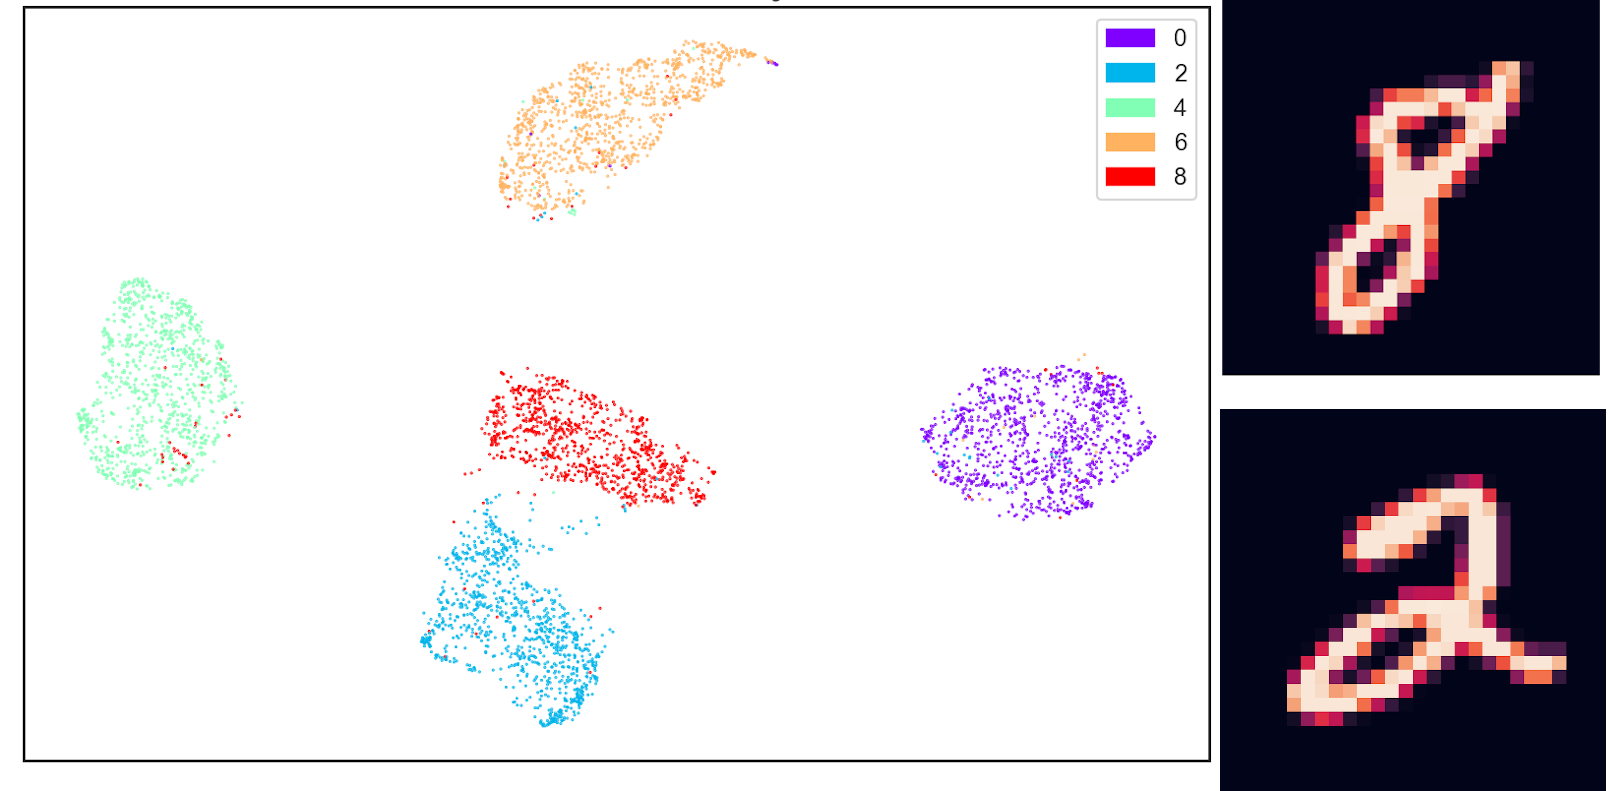
\includegraphics[width=13cm]{ODD.png}}
\end{center}
\caption{Left: 2D embedding of the first 10000 odd numbers of the MNIST dataset using UMAP reduction. The colormap represent the true digit category. Right: Examples of handwritten 2 and 8 digits form the MNIST database}
\label{fig:Odd}
\end{figure}
We can see on Figure \ref{fig:Odd} that most of the digits are well identified by this embedding. However, the cluster representing digits 2 and 8 are situated close together. This makes sense since those to digits are visually similar when handwritten (e.g. curvature) as shown on the right of Figure \ref{fig:Odd}.

\subsection{Embedding of the Iris Dataset}
\begin{figure}[!hbt]
\begin{center}
 \makebox[\textwidth]{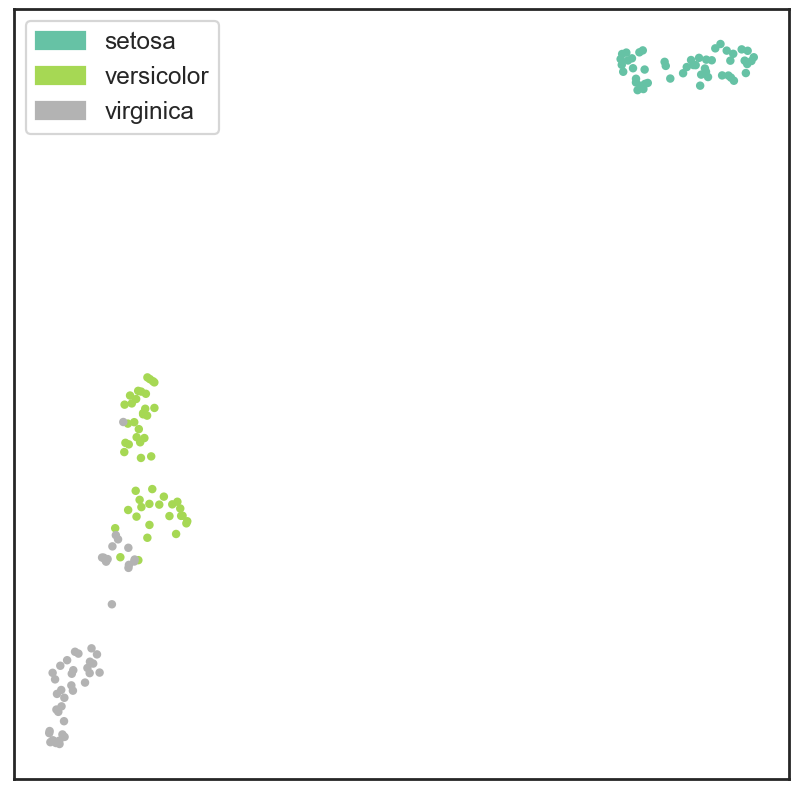
\includegraphics[width=6
 cm]{Iris.png}}
\end{center}
\caption{2D embedding of the iris dataset with a sample of 150 flowers using UMAP reduction. The colormap represent the true flower species.}
\label{fig:iris}
\end{figure}

As we can observe form Figure \ref{fig:iris}, the dimension reduction done on a combination of four features of the instances (the length and the width of the sepals, and the length and the width of the petals of the flower). The UMAP embedding does a relatively good job in distinguishing the species from each other even if the cluster representing the Iris versicolor and the Iris virginica are not always distinguishable.

\FloatBarrier

\section{Neural Network Classifier}
\subsection{MNIST Classification}

\begin{figure}[!hbt]
\begin{center}
 \makebox[\textwidth]{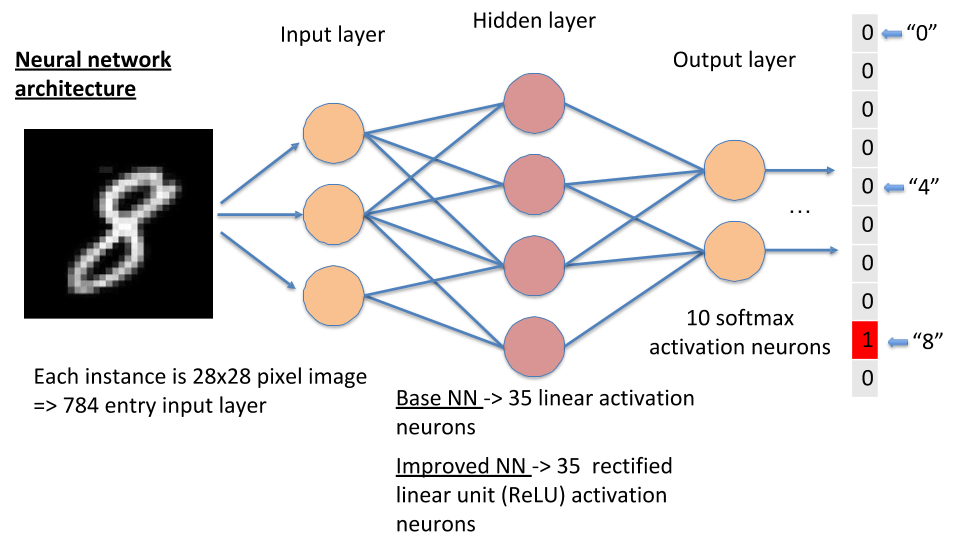
\includegraphics[width=8.5
 cm]{NN_archi.png}}
\end{center}
\caption{Visual representation of the neural network architectures}
\label{fig:NN}
\end{figure}

The improvements made to the base neural network was to: change the learning rate method for gradient descent from a fix to an adaptative one, change the activation of the dense layer node from a linear to a rectified linear unit function, augmenting the epochs, and reducing the batch size (see Table \ref{tab:NN} for full details).\par
The test accuracy was estimated via cross-validation where the dataset was splitted in 10 equal parts. The training was thus done on 9 parts while the test was done on the remaining part and this iteratively until each part was used in the test. The mean performance score was calculated by doing the average of all iteration's accuracy score. The base neural network performed a test accuracy of 75\% on the classification of 500 MNIST images, whereas the improved one had a 88\% test accuracy ($\pm$ 4\% standard deviation across splits) on the same sample and 93\% on the full MNIST dataset (70'000 images). Cross-validation is great for rather small datasets because it uses each instances in the training so nothing goes to waste and it also allows a more valid performance estimate.\par
Cire\c{s}an et al. (2012) have achieved a near human level of classification (99.8\%) of the handwritten digits MNIST database using a multi-column deep neural network architecture. This architecture, inspired by the microcolumns of neurons in the human cortex, averages the response from DNN columns into a single one.



\setlength{\tabcolsep}{20pt}
\begin{table}[!h]
\small
\caption{Parameters of the Neural Networks}
\begin{tabular}{lcc}
\toprule
\multicolumn{1}{c}{Parameter} &
\multicolumn{1}{c}{Base NN} &
\multicolumn{1}{c}{Improved NN}\\
\midrule
Nbr of Hidden Layer  & 1 & 1             \\
Nbr of Neuron per Hidden Layer  & 35 & 35  \\ Activation Function & Linear & ReLU       \\
Batch Size & 20 & 10                 \\
Epochs & 1 & 12                \\
Optimizer & RMSProp & Adadelta \\
Learning Rate & 0.001   & adaptative   \\
Mean Test Accuracy (500 images) &  0.75 & 0.88 \\
Duration in sec (500 images) & 14 & 39 \\
Mean Test Accuracy (70'000 images) & 0.90  &  0.93 \\
Duration in min (70'000 images) & 3 &   34 \\
\midrule
\end{tabular}
\label{tab:NN}
\end{table}

\textbf{References}\\
\small{Cire\c{s}an, D., Meier, U., & Schmidhuber, J. (2012, June). Multi-column deep neural networks for image classification. In \textit{2012 IEEE conference on computer vision and pattern recognition} (pp. 3642-3649). IEEE.}

\end{document}